%%% Research Diary - Entry
\documentclass[11pt,a4paper]{article}

% Working date: The date this entry is describing. Not necessary the date of last edit.
\newcommand{\workingDate}{\textsc{Meeting Notes -- @year $|$ @MONTH $|$ @dday}}

% Name and institution must preceed call to researchdiary.sty package
% \newcommand{\userName}{Pierre Bréchet}
% \newcommand{\institution}{TUM}

% The guts and glory
\usepackage{research_diary}
\usepackage{usrcmd}
\bibliography{bibliography}

% Begin document.
% Use \logoPNG or \logoEPS. If compiling with PDFTeX, use \logoPNG
\begin{document}
% \logoPNG

{\Huge @MONTH @day Meeting notes}

\section{Informative Regularization}
The informative variant primal reads

\begin{align}
    & \begin{array}{*2{>{\displaystyle}l}}
        \min_{G, Q_1} \min_{\gamma} &\Big\{\int_{\ZY}{\bkt{c(G(z), y) - Q_1(z_1, y)}\d \gamma(z, y)}  + \eps \R(\gamma) \\
                                    &+ \delta_{\set{\pf{G}{\zeta}}}\paren{\pf{( \proj{1} )}{\pf{(G, \id)}{\gamma}}} + \delta_{\set{\nu}}\paren{\pf{( \proj{2} )}{\pf{(G, \id)}{\gamma}}}\Big\} \\
                                    & + \lambda_1 \int_{\ZAX}{\exp{\frac{Q_1(z_1, y)}{\lambda_1}} \d \oprod{\zeta_1}{\nu} (z_1, y)}
                                    % + \delta\set{\pf{\proj{1}}{\pf{(G, \id)}{\gamma}} = \pf{G}{\zeta}} + \delta\set{\pf{\proj{2}}{\pf{(G, \id)}{\gamma}} = \nu} \\
        \end{array} \label{eqn:rem-q_1}\\
    \iff & \min_{G, Q_1} \W_{c - Q_1}^{\eps}(\pf{G}{\zeta}, \nu)+ \lambda_1 \int_{\ZAX}{\exp{\frac{Q_1(z_1, y)}{\lambda_1}} \d \oprod{\zeta_1}{\nu} (z_1, y)} \label{eqn:rem-c-q_1}\\
    \iff & \min_{G} \Wice(\pf{G}\zeta, \nu)
\end{align}

\begin{rems}
    \begin{enumerate}
        \item
            \eqref{eqn:rem-q_1} For the sake of brevity, $Q_1 \circ \projZAX(z, y)$ is written  $Q_1(z_1, y)$.
        \item
            \eqref{eqn:rem-c-q_1} For the sake of brevity, $c \circ (G, \id) - Q_1 \circ \projZAX$ is written $c - Q_1$.
    \end{enumerate}
\end{rems}

Optimal transport plan is recovered through
\begin{align}
    \label{eqn:primal-dual-info-rotgan}
    \radon{\gamma}{\zetaxnu}(z,y)
                      &=\exp\paren{\frac{D_1 \circ G(z) + D_2(y) - c(G(z), y) + Q_1(z_1, y)}{\eps}}  \\
                      % \frac{\posi{D_1 \circ G(z) + D_2(y) - c(G(z), y) + Q_1(z_1, y)}}{2\eps} & \text{if $\R = \Rtwo$}
              % \end{array} \right. \\
\end{align}
Leading to the general algorithm

\begin{equation}
    \label{eqn:dual-info-rotgan}
    \tag{IROTGAN}
    \begin{array}{c>{\displaystyle}l}
        \circled {1} &
        \begin{array}{*2{>{\displaystyle}l}}
            D_1, D_2 \assign \argmax_{D_1, D_2} & \int_{Z} {D_1 \circ G(z) \d \zeta(z)} + \int_{X}{D_2(y) \d
            \nu(y)} \\
            % & - \lambda_2 \int_{\ZBX}{\exp{\frac{-Q_2(z_2, y)}{\lambda_2}} \d \oprod{\zeta_2}{\nu}} \\
              & - \eps \int_{\ZX} {\exp{\frac{1}{\eps}(D_1 \circ G(z) + D_2 (y) - c(x, y) + Q_1(z_2, y))} \d \zetaxnu}
        \end{array} \\
        \circled{2}& \d \gamma = \radon{\gamma}{\zetaxnu}(z, y) \\
        \circled{3}& Q_1 \assign \argmin_{Q_1} \int_{\ZY}{  - Q_1\circ \projZAX(z, y)}\d \gamma(z, y)   + \lambda_1 \int_{\ZBX}{\exp{\frac{Q_1(z_1, y)}{\lambda_1}} \d \oprod{\zeta_1}{\nu}(z_1, y)}\\
        \circled{4}& G \assign \argmin_{G} \int_{\ZX}c(G(z), y) \d \gamma(z, y)
    \end{array}
\end{equation}

$Q_1$ learns how to reduce the cost (prefer the transportation) along the joint measures that bear an informative value.

The informative variant of Sinkhorn loss-like $\SLice$ is implemented as
\begin{align}
    &\min_{G} \SLice(\pf{G}{\zeta}, \nu) = 2 \cdot \Wice(\pf{G}{\zeta}, \nu) - \Wce(\pf{G}{\zeta}, \pf{G}{\zeta}) \\%- \Wce(\nu, \nu)
    \iff &\boxed{\min_{G} 2 \cdot \min_{Q_1}\set{ \W_{c - Q_1}^{\eps}(\pf{G}{\zeta}, \nu)+ \lambda_1 \int_{\ZAX}{\exp{\frac{Q_1(z_1, y)}{\lambda_1}} \d \oprod{\zeta_1 }{\nu (z_1, y)}}} - \Wce(\pf{G}{\zeta}, \pf{G}{\zeta})}
\end{align}

\begin{figure}[!htbp]
   \centering
\begin{subfigure}[t]{0.48\textwidth}
   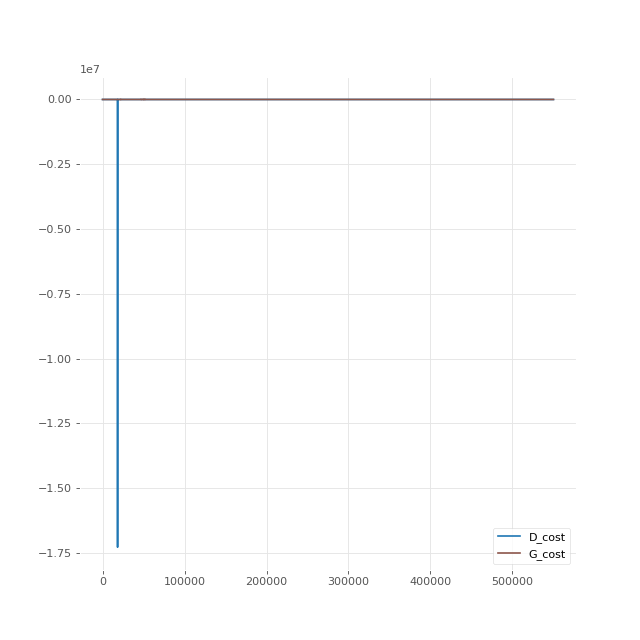
\includegraphics[width=\textwidth,center]{2019-04-30/mnist/info/plots/D_cost_G_cost.png}
   \caption{D_cost_G_cost.}
   \label{fig:.._.._notes_journal_figures_2019-04-30_mnist_info_plots-a}
\end{subfigure}
\begin{subfigure}[t]{0.48\textwidth}
   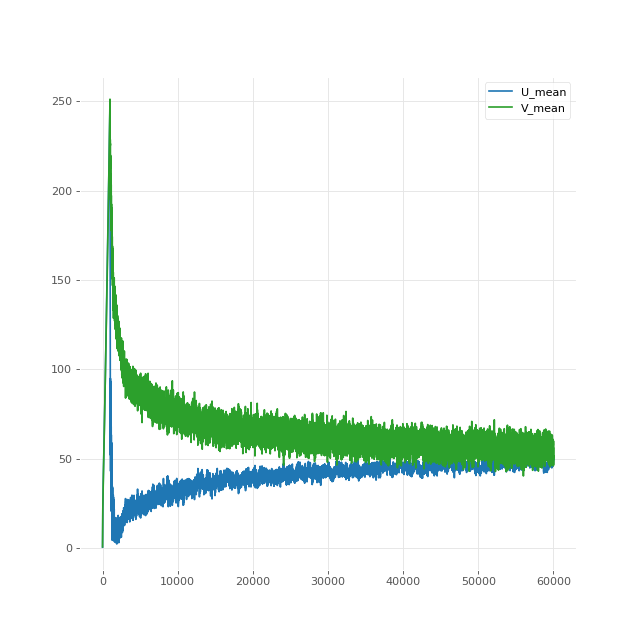
\includegraphics[width=\textwidth,center]{2019-04-30/mnist/info/plots/U_mean_V_mean.png}
   \caption{U_mean_V_mean.}
   \label{fig:.._.._notes_journal_figures_2019-04-30_mnist_info_plots-b}
\end{subfigure}
   \caption{.._.._notes_journal_figures_2019-04-30_mnist_info_plots}
   \label{fig:2019-04-30_mnist_info_plots}
\end{figure}
\begin{figure}[!htbp]
   \centering
\begin{subfigure}[t]{0.48\textwidth}
   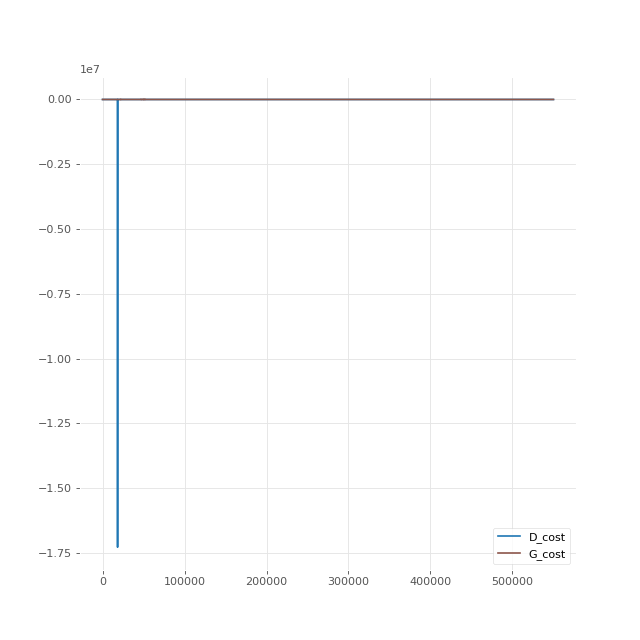
\includegraphics[width=\textwidth,center]{2019-04-30/mnist/info/plots/D_cost_G_cost.png}
   \caption{D_cost_G_cost.}
   \label{fig:.._.._notes_journal_figures_2019-04-30_mnist_info_plots-a}
\end{subfigure}
\begin{subfigure}[t]{0.48\textwidth}
   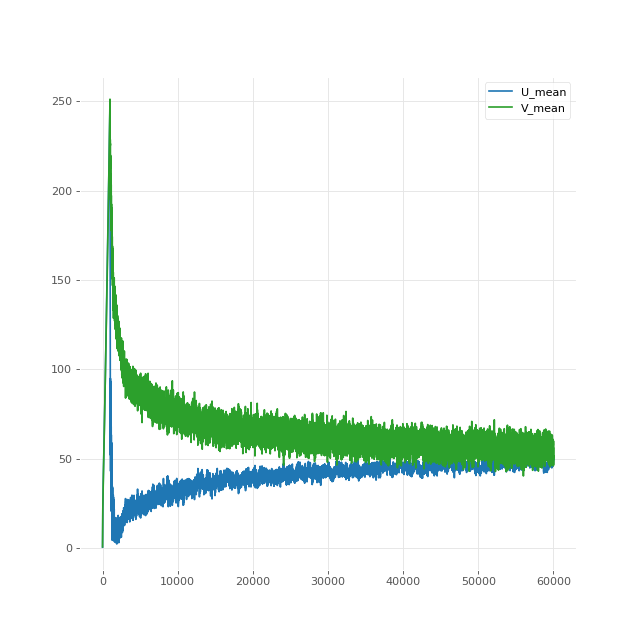
\includegraphics[width=\textwidth,center]{2019-04-30/mnist/info/plots/U_mean_V_mean.png}
   \caption{U_mean_V_mean.}
   \label{fig:.._.._notes_journal_figures_2019-04-30_mnist_info_plots-b}
\end{subfigure}
   \caption{.._.._notes_journal_figures_2019-04-30_mnist_info_plots}
   \label{fig:2019-04-30_mnist_info_plots}
\end{figure}

\section{Anti-informative Regularization}

The anti-informative primal reads
\begin{align}
    % \tag{Ent-ROTGAN}
    \label{eqn:anti-info-rotgan}
    % \tag{AROTGAN}
&\begin{array}{*2{>{\displaystyle}l}}
    \min_{G} \min_{\gamma}  &\int_{\ZY}{ c(G(z), y) \d \gamma(z, y)}  + \eps \R(\gamma)
    + \lambda_2 \KL{\pf{(\projZBX)}{\gamma}}{\oprod{\zeta_2}{\nu}}\\
                            &+ \delta_{\set{\pf{G}{\zeta}}}\paren{\pf{( \proj{1} )}{\pf{(G, \id)}{\gamma}}} + \delta_{\set{\nu}}\paren{\pf{( \proj{2} )}{\pf{(G, \id)}{\gamma}}}
\end{array} \\
    \iff & \min_{G} \Wace(\pf{G}{\zeta}, \nu)
    % \begin{split}
    % \min_{G} \min_{\gamma}  \int_{\ZY}{ c(G(z), y) \d \gamma(z, y)}  + \eps \R(\gamma)
    % + \lambda_2 \KL{\pf{(\projZBX)}{\gamma}}{\oprod{\zeta_2}{\nu}}\\
    %                    + \delta \set{\pf{\proj{1}}{\pf{(G, \id)}{\gamma}} = \pf{G}{\zeta}, \pf{\proj{2}}{\pf{(G, \id)}{\gamma}} = \nu}
    % \end{split}
\end{align}

\subsection{Primal update}

The $\min_{\gamma}\max_{Q_2}$ problem is convex in $\gamma$ and concave in $Q_2$. Therefore, the two operands can be switched, and the problem in $\gamma$ can be considered and solved for a fixed $Q_2$.

The optimal transport plan is learned as before
\begin{align}
    \label{eqn:primal-dual-info-rotgan}
    \radon{\gamma}{\zetaxnu}(z,y)
                      &=\exp\paren{\frac{D_1 \circ G(z) + D_2(y) - c(G(z), y) - Q_2(z_2, y)}{\eps}}
\end{align}

and $Q_2$ network is updated once $\gamma$ is found by maximizing the primal objective.

\begin{equation}
    \label{eqn:algo-1-anti-info-rotgan}
    \begin{array}{c>{\displaystyle}l}
        \circled {1} &
        \begin{array}{*2{>{\displaystyle}l}}
            D_1, D_2 \assign \argmax_{D_1, D_2} & \int_{Z} {D_1 \circ G(z) \d \zeta(z)} + \int_{X}{D_2(y) \d
            \nu(y)} \\
            % & - \lambda_2 \int_{\ZBX}{\exp{\frac{-Q_2(z_2, y)}{\lambda_2}} \d \oprod{\zeta_2}{\nu}} \\
              & - \eps \int_{\ZX}{\exp{\paren{ \frac{1}{\eps}(D_1 \circ G(z) + D_2 (y) - Q_2(z_2, y) - c(x, y)) }} \d \zetaxnu(z, y)}
        \end{array} \\
        \circled{2}& \d \gamma = \radon{\gamma}{\zetaxnu}(z, y) \\
        \circled{3}& Q_2 \assign \argmax_{Q_2} \int_{\ZY}{ Q_2 \circ \projZBX(z, y)}\d \gamma(z, y)   - \lambda_2 \int_{\ZBX}{\exp{\frac{Q_2(z_2, y)}{\lambda_2}} \d \oprod{\zeta_2}{\nu}(z_2, y)}\\
        \circled{4}& G \assign \argmin_{G} \int_{\ZX}c(G(z), y) \d \gamma(z, y)
    \end{array}
\end{equation}
% Therefore, the primal plan $\gamma$ learned differs for $\Wace(\pf{G}{\zeta}, \pf{G}{\zeta})$ and $\SLace(\nu, \nu) \neq 0$

\subsubsection{Corresponding Sinkhorn expression}

The anti-informative variant of Sinkhorn loss-like $\SLace$ is, in the context of primal update of $D_2$:
\begin{align}
    &\min_{G} \SLace(\pf{G}{\zeta}, \nu) = 2 \cdot \Wace(\pf{G}{\zeta}, \nu) - \Wce(\pf{G}{\zeta}, \pf{G}{\zeta}) \\%- \Wce(\nu, \nu)
    \iff &\min_{G} 2 \cdot \max_{Q_2}\set{ \W_{c + Q_2}^{\eps}(\pf{G}{\zeta}, \nu)- \lambda_2 \int_{\ZBX}{\exp{\frac{Q_2(z_2, y)}{\lambda_2}} \d \oprod{\zeta_2 }{\nu (z_2, y)}}} - \Wce(\pf{G}{\zeta}, \pf{G}{\zeta}) \label{eqn:rem-c-q_2}
\end{align}

test

\begin{figure}[!htbp]
   \centering
\begin{subfigure}[t]{0.48\textwidth}
   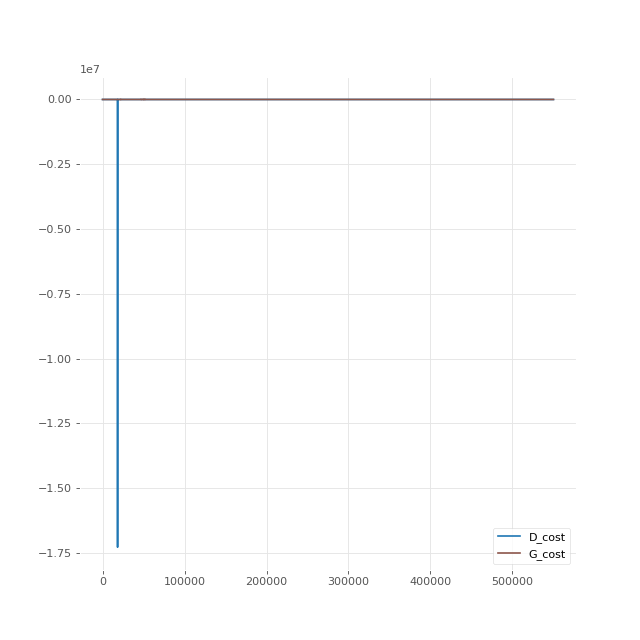
\includegraphics[width=\textwidth,center]{2019-04-30/mnist/info/plots/D_cost_G_cost.png}
   \caption{D_cost_G_cost.}
   \label{fig:.._.._notes_journal_figures_2019-04-30_mnist_info_plots-a}
\end{subfigure}
\begin{subfigure}[t]{0.48\textwidth}
   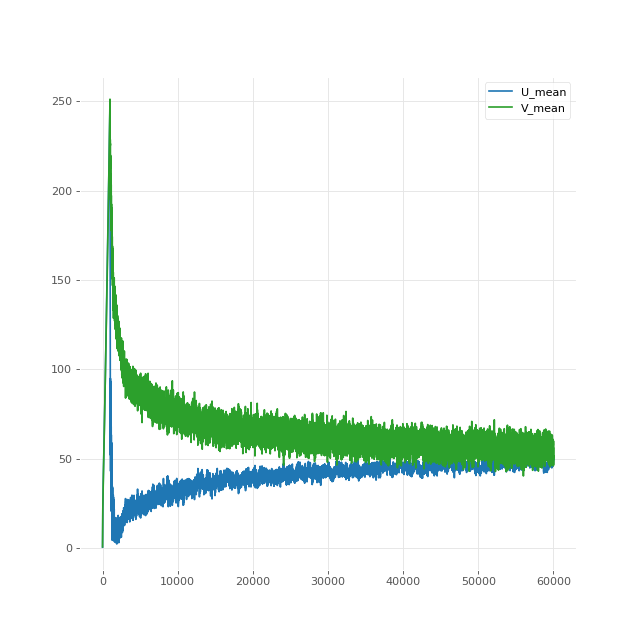
\includegraphics[width=\textwidth,center]{2019-04-30/mnist/info/plots/U_mean_V_mean.png}
   \caption{U_mean_V_mean.}
   \label{fig:.._.._notes_journal_figures_2019-04-30_mnist_info_plots-b}
\end{subfigure}
   \caption{.._.._notes_journal_figures_2019-04-30_mnist_info_plots}
   \label{fig:2019-04-30_mnist_info_plots}
\end{figure}

\begin{figure}[!htbp]
   \centering
\begin{subfigure}[t]{0.48\textwidth}
   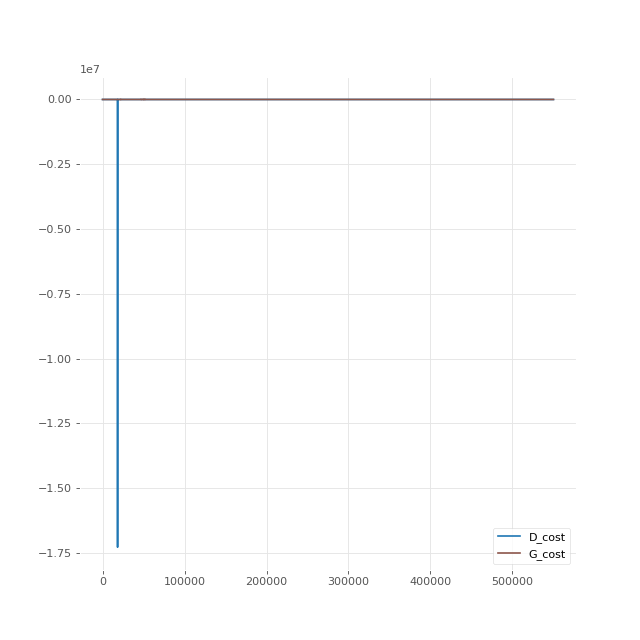
\includegraphics[width=\textwidth,center]{2019-04-30/mnist/info/plots/D_cost_G_cost.png}
   \caption{D_cost_G_cost.}
   \label{fig:.._.._notes_journal_figures_2019-04-30_mnist_info_plots-a}
\end{subfigure}
\begin{subfigure}[t]{0.48\textwidth}
   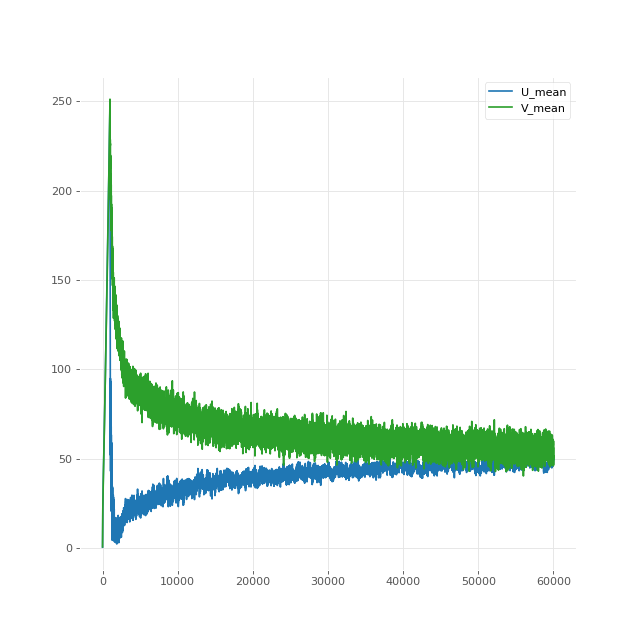
\includegraphics[width=\textwidth,center]{2019-04-30/mnist/info/plots/U_mean_V_mean.png}
   \caption{U_mean_V_mean.}
   \label{fig:.._.._notes_journal_figures_2019-04-30_mnist_info_plots-b}
\end{subfigure}
   \caption{.._.._notes_journal_figures_2019-04-30_mnist_info_plots}
   \label{fig:2019-04-30_mnist_info_plots}
\end{figure}

\subsection{Dual update}

The dual update of $Q_2$ is performed jointly with the dual variables $D_1, D_2$

\begin{equation}
    \label{eqn:dual-anti-info-rotgan}
    \begin{array}{c>{\displaystyle}l}
        \circled {1} &
        \begin{array}{*2{>{\displaystyle}l}}
            D_1, D_2, Q_2 \assign \argmax_{D_1, D_2, Q_2} & \int_{Z} {D_1 \circ G(z) \d \zeta(z)} + \int_{X}{D_2(y) \d
            \nu(y)} \\
                                                          & - \lambda_2 \int_{\ZBX}{\exp{\frac{Q_2(z_2, y)}{\lambda_2}} \d \oprod{\zeta_2}{\nu}} \\
              & - \eps \int_{\ZX}{\exp{\paren{ \frac{1}{\eps}(D_1 \circ G(z) + D_2 (y) - Q_2(z_2, y) - c(x, y)) }} \d \zetaxnu(z, y)}
            \end{array} \\
        \circled{2}& \d \gamma = \radon{\gamma}{\zetaxnu}(z, y) \\
        \circled{3}& G \assign \argmin_{G} \int_{\ZX}c(G(z), y) \d \gamma(z, y)
    \end{array}
    %     \begin{array}{*2{>{\displaystyle}l}}
    %         \eps \int_{\ZY}{\exp{\paren{\frac{D_1 \circ G(z) + D_2(y) - c(G(z), y) - Q_2(z_2,y)}{\eps}}} \d \zetaxnu(z, y)} &\text{if $\R = \Rent$} \\
    %         \frac{1}{2\eps} \int_{\ZY}{ \posi{D_1 \circ G (z) + D_2(y) - c(G(z), y) - Q_2(z_2,y)}^2 \d \zetaxnu(z, y)} & \text{if $\R=\Rtwo$}
    % \end{array} \right. \\
    %         &\eqdef \L_2(D_1, D_2, Q_2, G)
    %     \end{array}
\end{equation}
%\int_{X}u(x)\d \mu(x) + \int_{X}v(y) \d \nu(y) +
with

\begin{align}
    \label{eqn:primal-dual-anti-info-rotgan}
    \radon{\gamma}{\zetaxnu}(z,y)
                      &=\exp\paren{\frac{D_1 \circ G(z) + D_2(y) - c(G(z), y) - Q_2(z_2, y)}{\eps}}
\end{align}

\subsubsection{Corresponding Sinkhorn}

The anti-informative variant of Sinkhorn loss-like $\SLace$ is implemented, in the context of dual $D_2$, as
\begin{align}
    &\min_{G} \SLace(\pf{G}{\zeta}, \nu) = 2 \cdot \Wace(\pf{G}{\zeta}, \nu) - \Wce(\pf{G}{\zeta}, \pf{G}{\zeta}) \\%- \Wce(\nu, \nu)
    \iff &\boxed{\min_{G} 2 \cdot \int_{\ZX}c(G(z), y) \d \gammah(z, y) - \Wce(\pf{G}{\zeta}, \pf{G}{\zeta})}
\end{align}

\begin{rems}
    \begin{enumerate}
        \item \eqref{eqn:rem-c-q_2} For the sake of brevity, $c \circ (G, \id) + Q_2 \circ \projZBX$ is written $c + Q_2$.
            %         \item change $\Wce(\pf{G}{\zeta}, \pf{G}\zeta)$ to $\W_{c+Q_2}^{\eps}(\pf{G}{\zeta}, \pf{G}\zeta)$ ? would turn into
            %
            % \begin{align}
            %     &\min_{G} \max_{Q_2} 2 \cdot\W_{c + Q_2}^{\eps}(\pf{G}{\zeta}, \nu)- \W_{c+Q_2}^{\eps}(\pf{G}{\zeta}, \pf{G}\zeta) - \lambda_2 \int_{\ZBX}{\exp{\frac{Q_2(z_2, y)}{\lambda_2}} \d \oprod{\zeta_2 }{\nu (z_2, y)}} \\
            %     \iff & \min_{G}\max_{Q_2} 2 \cdot \SL_{c+Q_2}^{\eps}(\pf{G}{\zeta}, \nu)- \lambda_2 \int_{\ZBX}{\exp{\frac{Q_2(z_2, y)}{\lambda_2}} \d \oprod{\zeta_2 }{\nu (z_2, y)}}
            % \end{align}
    \end{enumerate}
\end{rems}

\begin{figure}[!htbp]
   \centering
\begin{subfigure}[t]{0.48\textwidth}
   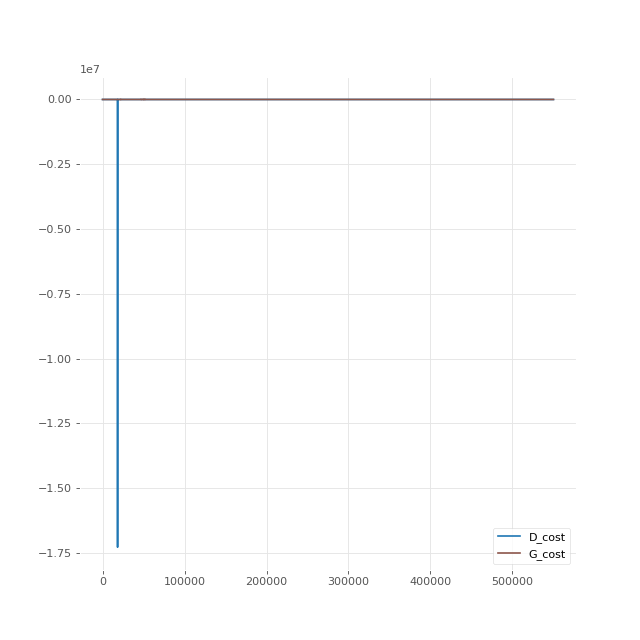
\includegraphics[width=\textwidth,center]{2019-04-30/mnist/info/plots/D_cost_G_cost.png}
   \caption{D_cost_G_cost.}
   \label{fig:.._.._notes_journal_figures_2019-04-30_mnist_info_plots-a}
\end{subfigure}
\begin{subfigure}[t]{0.48\textwidth}
   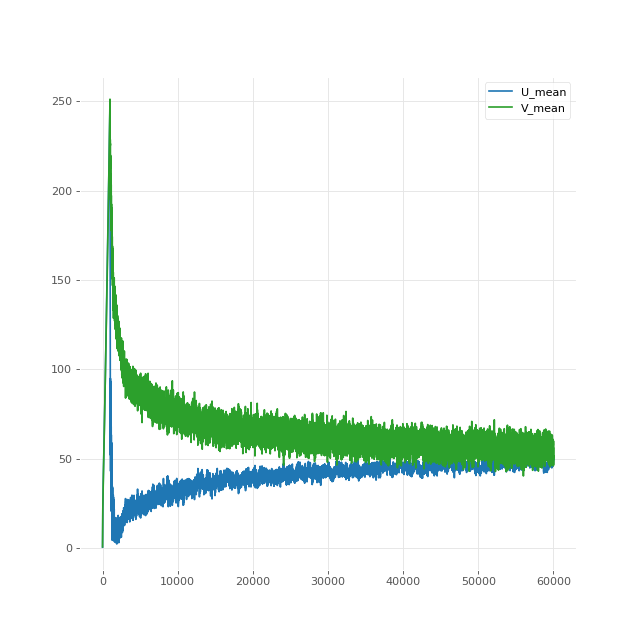
\includegraphics[width=\textwidth,center]{2019-04-30/mnist/info/plots/U_mean_V_mean.png}
   \caption{U_mean_V_mean.}
   \label{fig:.._.._notes_journal_figures_2019-04-30_mnist_info_plots-b}
\end{subfigure}
   \caption{.._.._notes_journal_figures_2019-04-30_mnist_info_plots}
   \label{fig:2019-04-30_mnist_info_plots}
\end{figure}

\begin{figure}[!htbp]
   \centering
\begin{subfigure}[t]{0.48\textwidth}
   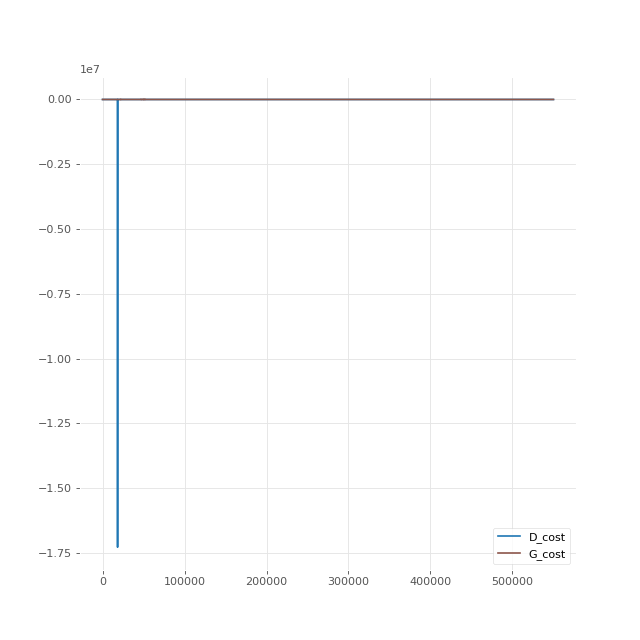
\includegraphics[width=\textwidth,center]{2019-04-30/mnist/info/plots/D_cost_G_cost.png}
   \caption{D_cost_G_cost.}
   \label{fig:.._.._notes_journal_figures_2019-04-30_mnist_info_plots-a}
\end{subfigure}
\begin{subfigure}[t]{0.48\textwidth}
   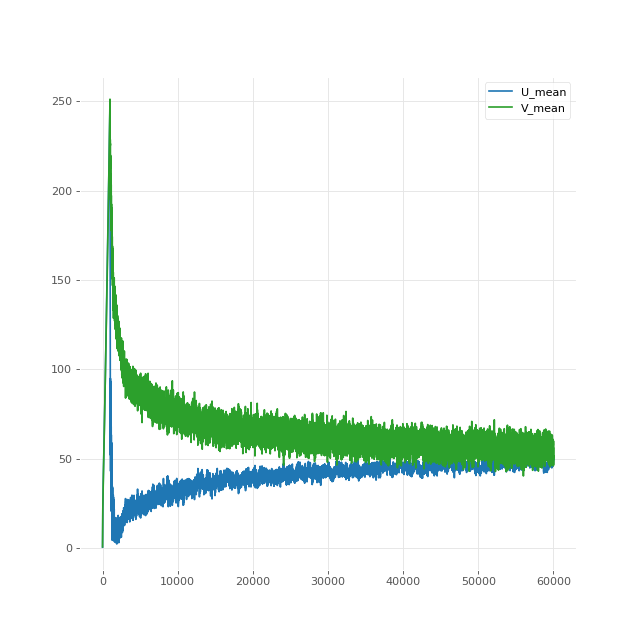
\includegraphics[width=\textwidth,center]{2019-04-30/mnist/info/plots/U_mean_V_mean.png}
   \caption{U_mean_V_mean.}
   \label{fig:.._.._notes_journal_figures_2019-04-30_mnist_info_plots-b}
\end{subfigure}
   \caption{.._.._notes_journal_figures_2019-04-30_mnist_info_plots}
   \label{fig:2019-04-30_mnist_info_plots}
\end{figure}

\section*{After the meeting}
\begin{itemize}
    \item
        Focus on models that are promising
    \item
        Try modifying the cost with $Q_1$ in the update of the informative sinkhorn model
    \item
        Results of  the informative model without sinkhorn
    \item
        Theoretical analysis of the informative model with Sinkhorn is difficult with the concave / convex problem. Would be easier with the anti-informative (since the primal remains convex). amd the principled formulation requires an additional $Q$ network.
    \item
        (strong) convexity of the informative formulation, with eigen values of the linear operator mapping the transport plan (marginalization)? if integration on a compact, the integral would be bounded $\leadsto$ bounded linear operator. Nature of $\eps g - \lambda g(Ax)$ for $g$ convex ?
    \item
        Sinkhorn loss aims at unbiasing the primal cost. Introducing informative regularization might already unbias the transport plan ? Along the informative latent dimension. Anti-informative regularization might increase the bias (on the noisy latent diemnsions). Principled way to derive the Sinkhorn loss in the context of informative regularized models is still open.
    \item
        For CelebA simply use one thread.
\end{itemize}

\printbibliography{}
\end{document}
